\section{TCP versions}

\subsection{TCP Tahoe}
One of the first protocols, very basic. It uses the Slow Start Phase and 
AIMD, but it only relies on timeouts to detect losses, so no fast retransmit nor 
fast recovery (it doesn't check for dupacks). At every loss, it always restart 
from 1.

\paragraph*{Characteristics}
\begin{itemize}
  \item Standard TCP functions
  \item ``Slow'' start
  \item Congestion control: AIMD, only timeouts to detect losses (no dupacks)
\end{itemize}

\begin{figure}[h]
  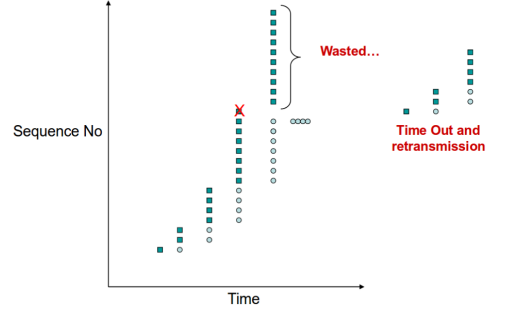
\includegraphics[scale=0.8]{tahoe}
  \caption[TCP Tahoe]{TCP Tahoe uses only timeouts to detect losses}
\end{figure}

\subsection{TCP Reno}
\paragraph*{Characteristics}
\begin{itemize}
  \item Fast Retransmit/Fast Recovery (3 dupAcks to recover one packet loss)
  \item TCP Reno can recover from one packet loss without having a time out
\end{itemize}

\begin{figure}[h]
  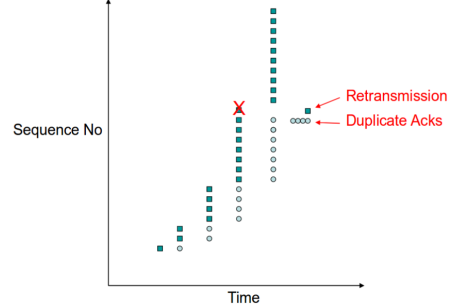
\includegraphics[scale=0.8]{fast_retransmit}
  \caption[TCP Reno 1]{TCP Reno - Fast Retransmission}
\end{figure}

\begin{figure}[h]
  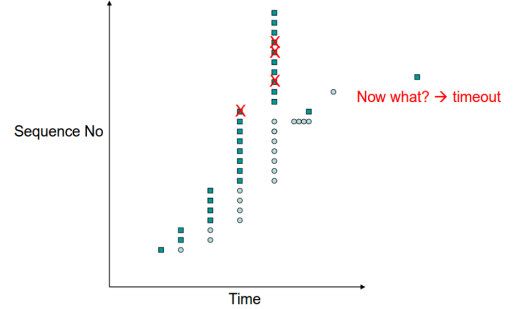
\includegraphics[scale=0.8]{reno}
  \caption[TCP Reno 2]{TCP Reno - more than one packet loss}
\end{figure}

\subsubsection{TCP New Reno}
TCP New Reno introduces partial ACKs to recover more packets without the use of
timeouts.
\begin{figure}[h]
  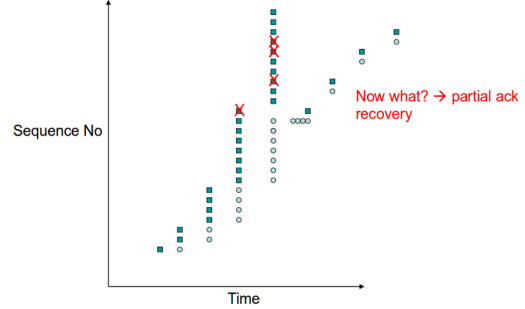
\includegraphics[scale=0.8]{partial_acks}
  \caption[TCP New Reno]{TCP New Reno - partial ACKs}
\end{figure}

\subsection{TCP SACK}
SACK means \textit{Selective acknowledgment}. This means that all ACKs are a
little bigger but carry more information, they can give the sender the complete 
picture.

Returning ACKs declares which packets (even non contiguous) were received.
All non-received packets can be retransmitted and so it recovers from multiple
losses in just one RTT.
\begin{figure}[h]
  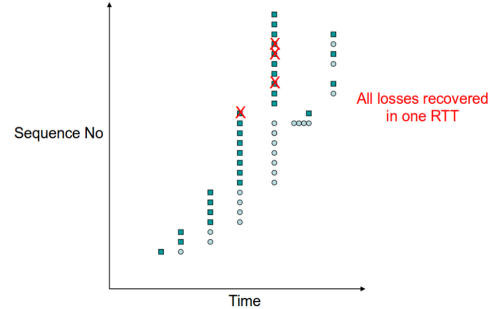
\includegraphics[scale=0.8]{sack}
  \caption[TCP SACK]{TCP SACK - Recovery from multiple losses in just one RTT}
\end{figure}

\subsubsection{Differences between TCP New Reno and TCP SACK}

TCP New Reno works by assuming that the packet that immediately follows the partial ACK received at fast recovery is lost, and retransmit
the packet. However, this might not be true and it affects the performance of TCP. SACK TCP adds a number of SACK blocks in TCP packet,
where each SACK block acknowledges a non-contiguous set of data has been received. The main difference between SACK TCP and Reno TCP
implementations is in the behavior when multiple packets are dropped from one window of data. SACK sender maintains the information which
packets is missed at receiver and only retransmits these packets. When all the outstanding packets at the start of fast recovery are
acknowledged, SACK exits fast recovery and enters congestion avoidance.\footnote{
  \url{http://www.roman10.net/2011/11/10/tcp-tahoe-reno-newreno-and-sacka-brief-comparison/}
}

\begin{figure}[h]
  \centering
  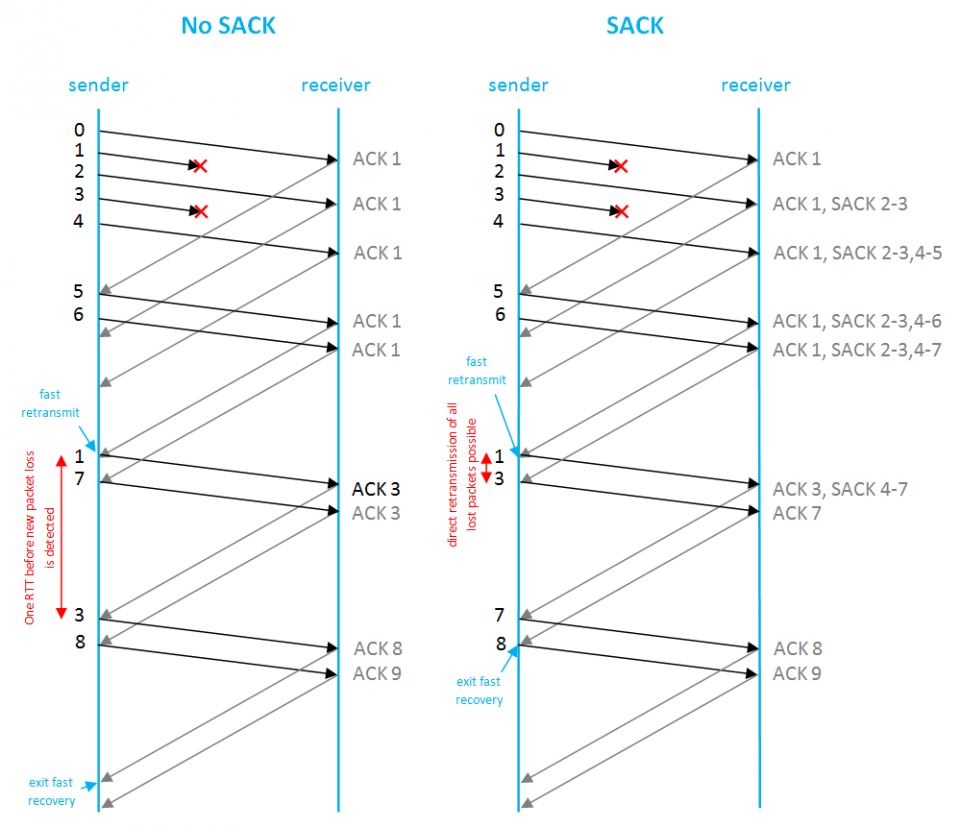
\includegraphics[scale=0.33]{TCPFlowSackNoSack}
  \caption[TCP No SACK vs TCP SACK]{A comparison between TCP SACK versus one without SACK}
  \label{fig:tcp:sackvsnosack}
\end{figure}
